% !TEX root = ../main.tex
\section{Branch and bound elimination in the reduced domain}\label{sec:branch-and-bound-elimination-in-the-reduced-domain}

To rule out fit throughout $D$, we examine whole regions of configurations
at a time. Each successful component must rule out fit for every configuration in
the region that belongs to $D$. We subdivide unresolved regions, seeking a
resolution high enough for at least one component to eliminate them.
The proof rests on two facts about the result: every region was eliminated
soundly, and the eliminated regions cover $D$.
\Cref{sec:generating-and-verifying-the-certificate} checks both for the
final certificate and lists everything the proof relies on. The notions of
range and completion in \cref{subsec:component-hierarchy} explain why the
subdivision finishes and how the components were found; the proof itself
does not use them.

\subsection{Boxes, subdivision, and elimination}\label{subsec:boxes-subdivision-and-elimination}

A \emph{box} is a Cartesian product of closed parameter intervals,
\[
  B=\prod_{i=1}^{5}[l_i,h_i]\subseteq B_0,
  \qquad l_i,h_i\in\mathbb Q,\quad l_i\le h_i,
\]
in the coordinate order $s,t,r_1,r_2,r_3$. Each point of $B$ represents a
configuration. Rational endpoints allow the box itself
to be recorded exactly. The boxes created by our search have positive
width in every coordinate, so they cover entire five-dimensional regions
of configuration space.

We \emph{eliminate} a box when we certify that it contains no fit
configuration in $D$. In terms of the margin, the required conclusion is
\begin{equation}\label{eq:box-elimination}
  M_{\mathcal R}(c)\ge1\qquad\text{for all }c\in B\cap D.
\end{equation}
A component takes a box and attempts to justify its elimination. If it
succeeds, we store a \emph{certificate record} identifying the box, the
successful component and the data needed to verify its result. Otherwise,
its answer is inconclusive.
A component is \emph{sound} if every accepted result establishes
\cref{eq:box-elimination}.
In particular, elimination allows touch configurations, and a box disjoint
from $D$ satisfies this condition without any geometric comparison.

\paragraph{Subdivision.}
We call a set of components used together for elimination a \emph{collection}.
The procedure starts with $B_0$. For each unresolved box, it tries the
members of the collection in a fixed order, stopping at the first successful one. If none
succeeds, it bisects one of the intervals at its midpoint
$m=(l_i+h_i)/2$, replacing $[l_i,h_i]$ by $[l_i,m]$ and $[m,h_i]$ while
leaving the other four intervals unchanged. Both children are closed,
axis-parallel boxes containing the four-dimensional dividing face, and
their union is exactly the parent box.

The number of bisections from $B_0$ to a box is its \emph{depth}. We bisect
coordinates cyclically in the order $s,t,r_1,r_2,r_3$, and process boxes in
increasing depth. Boxes that remain unresolved are therefore refined adaptively
to arbitrarily small widths in all five coordinates. The decision to subdivide depends on
whether a box has been eliminated; the coordinate order does not.

\paragraph{Complete coverage.}
An important invariant is that the eliminated boxes together with the unresolved
boxes always cover $B_0$. This holds initially and is preserved both when a box is
eliminated and when it is replaced by its two children. Consequently, if
the procedure finishes with finitely many eliminated boxes and none
unresolved, their certificate records form a complete certificate of
non-Rupertness. Indeed, a fit would have a representative in $D$
by \cref{prop:representative-coverage}. That representative would belong
to an eliminated box, contradicting \cref{eq:box-elimination}. Shared
boundaries introduced by the bisections cause no exception to this reasoning.

This explains what completion would prove; it does not yet show that the
collection will resolve every box. Stopping at a time or depth limit leaves
the unresolved regions to be treated. \Cref{sec:generating-and-verifying-the-certificate}
describes how these records and their coverage are checked.

For convex polyhedra with algebraic vertex coordinates,
\citet{SteiningerYurkevich2023} give the theoretical decision procedure
discussed in \cref{subsec:previous-approaches-and-the-remaining-difficulty}.
Their procedure reduces
the problem to solving systems of polynomial equations and inequalities,
but they regard the resulting computations as impractical. Our aim is to
develop a collection that uses the geometric properties of the RID
to make certificate generation feasible.

\subsection{Component hierarchy}\label{subsec:component-hierarchy}

Even though components are applied to entire boxes, their usefulness and
scope can be better understood by considering individual configurations.
If a component works uniformly throughout some neighbourhood
around a configuration, it will generally handle sufficiently small boxes
there. We make this connection precise so that later descriptions of where
a component applies have a common and unambiguous meaning.

Call any box obtainable by the cyclic midpoint subdivision of $B_0$ a
\emph{search box}, whether or not a particular run reaches it. Neighbourhoods
below are relative to $B_0$: at its boundary, only configurations inside
$B_0$ need to be considered. Distances and diameters refer to Euclidean
distance between the five parameter coordinates.

\begin{lemma}[Search boxes in neighbourhoods]\label{lem:search-boxes-in-neighbourhoods}
  Every configuration $c\in B_0$ belongs to a search box at every depth.
  For any neighbourhood $U$ of $c$ relative to $B_0$, all sufficiently deep
  search boxes containing $c$ lie entirely in $U$. In particular, every
  nonempty relatively open subset of $B_0$ contains a search box.
\end{lemma}
\begin{proof}
  The full subdivision at each depth covers $B_0$, since the two closed
  children cover their parent. At depth $d$, each coordinate has been
  bisected at least $\lfloor d/5\rfloor$ times, so every search box at that
  depth satisfies
  \begin{equation}\label{eq:search-box-diameter-bound}
    \operatorname{diam}B
      \le 2^{-\lfloor d/5\rfloor}\operatorname{diam}B_0.
  \end{equation}
  Choose $\varepsilon>0$ such that every point of $B_0$ at distance less
  than $\varepsilon$ from $c$ belongs to $U$. For sufficiently large $d$,
  this diameter bound is less than $\varepsilon$, so every point of a
  search box containing $c$ belongs to $U$. The argument also applies
  when $c$ lies on a boundary of $B_0$ or a subdivision face.
\end{proof}

\begin{definition}[Range of a component]\label{def:range-of-a-component}
  A configuration $c\in B_0$ belongs to the \emph{range} of a component if
  it has a neighbourhood $U$ in $B_0$ such that the component accepts every
  search box $B\subseteq U$. The range of a collection is
  defined in the same way, allowing any member to accept
  each such box.
\end{definition}

Acceptance here means that the component's check succeeds, including any
selection of the data needed for its certificate record. A box does not count
as accepted just because a valid record exists; the component must find and
verify one. Different boxes may use different data in their records, or
different members of a collection. This definition describes an open region
relative to $B_0$.

In particular, accepting one closed box with $c$ on its boundary does not
establish that $c$ lies in the component's range. Smaller boxes around $c$
can extend across that boundary. The same issue arises where two proved
regions meet: a box extending across both regions needs a component that can
certify all of it. A component may check that the box is covered by a union of already
proved regions, or another component may handle the whole box. Acceptance
of only the box's centre is not enough.

\begin{lemma}[Finite completion from local coverage]\label{lem:finite-completion-from-local-coverage}
  Suppose the range of a fixed finite collection covers $B_0$, all its
  members are sound, and every component call finishes. Then the increasing-depth search
  with cyclic midpoint subdivision terminates after finitely many boxes,
  provided no time or depth limit stops it.
\end{lemma}
\begin{proof}
  Around each configuration in $B_0$, choose a ball of radius $2\varepsilon$, with
  $\varepsilon>0$, whose intersection with $B_0$ lies in an accepting
  neighbourhood. The balls with radii $\varepsilon$ still cover $B_0$.
  Compactness gives a finite subcover; let $\delta>0$ be the smallest
  radius in that finite subcover.

  Any search box of diameter less than $\delta$ lies in one of the
  corresponding larger balls. Indeed, choose a point of the box and a
  smaller ball containing it. Every other point of the box is within
  $\delta$ of that point, hence within twice the smaller ball's radius
  of its centre. Such a box is therefore accepted.

  By \cref{eq:search-box-diameter-bound}, at sufficiently large finite
  depth every search box has diameter less than $\delta$, so every box
  at that depth is accepted without further subdivision.
  There are only finitely many boxes up to that depth, and processing each
  one takes finitely many component calls, all of which finish. The search
  therefore terminates.
\end{proof}

\paragraph{Developing the collection.}
The same finite-cover reasoning applies to any compact subset of the
collection's range: sufficiently small unresolved boxes cannot continue
to meet that subset. Refinement can therefore help locate the configurations
for which further components are needed. Small changes in the margin alone
do not establish this property; we must show that the relevant component
actually succeeds on the nearby boxes.

This gives a way to develop the collection successively. When refinement
concentrates on configurations the current collection cannot handle, we
examine their geometry and add a component to handle them. Each addition works
alongside the preceding components. The need to treat aligned configurations
was already apparent before running the Global component, which detects
protrusion: at an aligned configuration the shadows coincide, so no
projected plug vertex protrudes beyond the hole's shadow.

The final collection has four components, in the order in which we develop
them: the \emph{Domain} component (\cref{subsec:domain-component-skipping-boxes-outside-the-reduced-domain}),
which discards boxes outside $D$; the \emph{Global} component
(\cref{sec:global-component}), for poke configurations; the \emph{Local}
component (\cref{sec:local-component}), for neighbourhoods of aligned
configurations; and the \emph{Exotic} component
(\cref{sec:square-and-pentagon-configurations,sec:arc-configurations,sec:endpoint-and-crossing-configurations}),
with eight covers around the remaining touch configurations.
\Cref{fig:hierarchy} shows how each addition clears boxes that the
preceding components leave unresolved. The program may try an inexpensive
specialised check before a more general one; the order affects only which
record a box receives.

\begin{figure}[htbp]
\centering
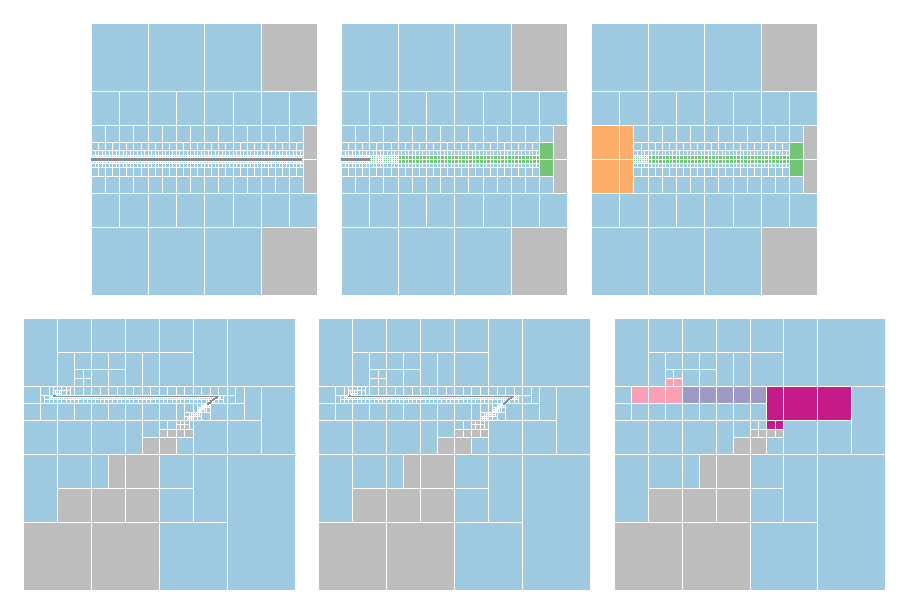
\includegraphics[width=\linewidth]{figures/hierarchy}
\caption{The collection built up component by component on two planes of configurations, each halved alternately until a component eliminates a piece or the piece is $16$ (top) or $18$ (bottom) halvings deep; pieces still unresolved at that depth are black. Top: the plane $t=0$, $r_1=r_2=0$ through the square configuration, with $s\in[0,2/3]$ horizontally and $r_3\in[-2/5,2/5]$ vertically. Bottom: the plane $\Pi_1$ of \cref{sec:arc-configurations}, with $s\in[3/16,5/8]$ horizontally and $\theta\in[-5/16,1/8]$ vertically. Left: the \fc{Domain}{Domain (grey)} and \fc{Global}{Global (light blue)} components leave the aligned configurations $r_3=0$ and the two arcs unresolved. Middle: the \fc{Local}{Local component (green)} eliminates the aligned configurations except near the square configuration $s=0$, and nothing on the arcs. Right: the whole collection, which leaves nothing; the Exotic covers (\fc{Square}{square light orange}, \fc{Arc}{arc lavender}, \fc{Endpoint}{endpoint light pink}, \fc{Crossing}{crossing magenta}) are tried before the Local component, so the square cover also takes pieces that the Local component would eliminate.}
\label{fig:hierarchy}
\end{figure}

\subsection{\emph{Domain} component: skipping boxes outside the reduced domain}\label{subsec:domain-component-skipping-boxes-outside-the-reduced-domain}

The simplest component uses the inequalities defining $D$ in
\cref{eq:reduced-domain}. If one of them is strictly violated throughout
$B$, then $B\cap D=\varnothing$. We call this the \emph{Domain} component.
The justification is the representative-coverage result: the configurations
discarded here already have representatives in $D$. They need not be poke configurations.

\paragraph{Affine inequalities.}
The viewing-triangle inequality and the twelve relative-rotation inequalities
are affine. Write one as $p(c)\le0$, subtracting its right side from its
left side. To minimise $p$ on $B$, choose the lower endpoint in every
coordinate with a positive coefficient and the upper endpoint for a negative
coefficient; a zero coefficient permits either choice. This gives the exact
minimum. If it is strictly positive, the entire box violates the inequality.
Equality is insufficient because the inequalities defining $D$ are
non-strict.

\paragraph{Fold inequalities.}
The fold inequalities require more care. A \emph{corner} of a box is
obtained by choosing an endpoint of each parameter interval. We group
these choices according to what they control. The allowed pairs $(s,t)$
fill a rectangle in the $(s,t)$-plane, which we call the \emph{viewing
rectangle}. Choosing an endpoint for each of $s$ and $t$ gives its four
corners, each specifying a viewing direction. Independently, the allowed
vectors $\mathbf r=(r_1,r_2,r_3)$ fill a three-dimensional \emph{rotation box},
whose eight corners choose an endpoint for each of $r_1,r_2,r_3$. Each viewing
corner can be combined with any rotation corner, giving the $4\times8=32$
corner configurations of $B$.

The square of an expression can be large at both ends of an
interval while the expression changes sign and vanishes inside. For this
reason, evaluating only the squared fold inequalities at the corners would
not justify eliminating the box. We also check the sign before squaring.

\begin{proposition}[Whole-box fold violation]\label{prop:whole-box-fold-violation}
  Fix $g\in\mathcal Q_+$. The inequality
  \[
    {\ell_g(c)}^2>1+s^2+t^2
  \]
  holds throughout $B$ if and only if it holds at every corner of $B$
  and the values of $\ell_g$ at all corners have one common nonzero sign.
\end{proposition}
\begin{proof}
  Suppose first that the corner conditions hold, and let
  $\sigma\in\{-1,1\}$ be the common sign. At every corner,
  \[
    \sigma\ell_g(c)-\lVert\mathbf u\rVert>0,
    \qquad\mathbf u=(s,t,1).
  \]
  Fix $\mathbf r$ at one of the eight rotation corners. The expression $\ell_g$ is
  affine in $(s,t)$, as follows from the quaternion product in
  \cref{eq:fold-polynomial}.
  The norm of $(s,t,1)$ is convex, so the displayed difference is
  concave in $(s,t)$. Every pair $(s,t)$ in the viewing rectangle is a convex
  combination of its four corners. Concavity therefore makes the difference
  at least the corresponding combination of four strictly positive values.
  It is strictly positive throughout that rectangle.

  This holds for each rotation corner. Now fix arbitrary
  $(s,t)\in[l_1,h_1]\times[l_2,h_2]$.
  The same difference is affine in $\mathbf r$, so interpolation between
  the eight rotation corners proves strict positivity throughout the
  rotation box. Thus $\sigma\ell_g(c)>\lVert\mathbf u\rVert>0$ everywhere
  in $B$, and squaring proves the required inequality.

  Conversely, if the inequality holds throughout $B$, then
  $|\ell_g(c)|>\lVert\mathbf u\rVert\ge1$. The continuous function
  $\ell_g$ cannot change sign on the connected box without vanishing.
  Its corner values consequently have the same nonzero sign and satisfy
  the strict inequalities. The proof also applies to zero-width intervals,
  where some of the corner choices coincide.
\end{proof}

\paragraph{Checking a box in the implementation.}
The implementation writes every inequality defining $D$ in the form
$q(c)\le0$ for a polynomial $q$: the affine inequalities as above, and
each fold inequality as $q={\ell_g}^2-(1+s^2+t^2)$. To eliminate $B$, it
certifies $q>0$ throughout $B$ by applying the Bernstein sign test of
\cref{subsec:bernstein-coefficients} to $-q$. For an affine inequality the
coefficients are exactly the corner values, so this is the endpoint rule
above. For a fold inequality it is a sufficient condition, and
\cref{prop:whole-box-fold-violation} describes exactly when a box violates
the inequality throughout. The component tries only the inequalities
whose value at the midpoint of the box, computed in floating point, is
positive. An inequality that holds at the midpoint cannot be violated
throughout the box, and a rounding error in this choice can only leave a
box unresolved; the elimination itself rests on the exact test.

All the corner values and coefficients lie in $\mathbb Q(\sqrt5)$, since
the box endpoints are rational and the coefficients lie in that field.
Their exact signs can be determined using integers;
\cref{subsec:exact-representation-of-field-elements-with-integers}
gives these operations in the next section.
A certificate record produced by the Domain component identifies the domain
inequality violated throughout the box, so its checker can reconstruct and
repeat the whole-box test.

If none of the tests succeeds, the box may still be disjoint from $D$:
different parts of it could violate different inequalities. Further
subdivision can separate those parts. In particular, every point of
$B_0\setminus D$ strictly violates at least one defining inequality.
Continuity preserves that violation in a closed neighbourhood, and the
exact test accepts every sufficiently small box contained in it, by the
convergence of Bernstein coefficients proved in
\cref{lem:convergence-of-bernstein-coefficients}. Thus the Domain
component handles sufficiently small boxes around every point outside $D$. Configurations on
the retained boundary still require the geometric components. Before
developing those components, we explain how to carry out these calculations
exactly and certify the sign of more general polynomials on a box.
